%-------------------------------------STYLES----------------------------------------------------------------%

\documentclass[10pt, xcolor=dvipsnames]{beamer}

%\mode<presentation>
%{
\usetheme{Madrid}
%\setbeamercovered{transparent}
%} 
%\usefonttheme{professionalfonts}
\usecolortheme{beaver}

\usepackage{setspace}
\usepackage[english]{babel}
\usepackage[latin1]{inputenc}
\usepackage{times}
\usepackage[T1]{fontenc}
\usepackage{color}
\usepackage{graphicx}
\usepackage{amssymb}
\usepackage{amsthm}
\usepackage{bm}
\usepackage{rotating}
\usepackage{ccaption}
\usepackage{booktabs}
\usepackage{lscape}
\usepackage{colortbl}
\usepackage{arydshln}
\usepackage{tabularx}
\usepackage{appendixnumberbeamer}

%\useinnertheme{rounded}
\setbeamertemplate{items}[balls]
%\usepackage[notocbib]{apacite}                % This is bibliography package.
%\renewcommand{\bibliographytypesize}{\tiny}
\setbeamertemplate{navigation symbols}{}
\usepackage{graphics}
\usepackage{epstopdf}
\DeclareGraphicsRule{.tif}{png}{.png}{`convert #1 `dirname #1`/`basename #1 .tif`.png}
%\usepackage{fleqn}
%\setlength{\mathindent}{1cm}
%\color{white}
%\hypersetup{colorlinks=true,linkcolor=Blue}
\usepackage{bbm}
\newcommand{\backupbegin}{
   \newcounter{framenumberappendix}
   \setcounter{framenumberappendix}{\value{framenumber}}
}
\newcommand{\backupend}{
   \addtocounter{framenumberappendix}{-\value{framenumber}}
   \addtocounter{framenumber}{\value{framenumberappendix}}
}

%% Change the margins
\newenvironment{changemargin}[2]{%
  \begin{list}{}{%
    \setlength{\topsep}{0pt}%
    \setlength{\leftmargin}{#1}%
    \setlength{\rightmargin}{#2}%
    \setlength{\listparindent}{\parindent}%
    \setlength{\itemindent}{\parindent}%
    \setlength{\parsep}{\parskip}%
  }%
  \item[]}{\end{list}}

\newtheorem{proposition}{Proposition}

%-------------------------------------------Title---------------------------------------------------%


\title[Land Constraints]{{The Role of Land in Temperate and Tropical Agriculture}}

\author[Johnson \& Vollrath]{T. Ryan Johnson \inst{1} \and Dietrich Vollrath \inst{2}}
\institute[UH]{\inst{1} Washington University \and %
                      \inst{2} University of Houston}

\date[November 2018]{}

%-------------------------------------------Slides---------------------------------------------------%

\begin{document}
\maketitle

\section{Introduction}

\begin{frame}{The basic questions}\label{define}

What is the elasticity of agricultural output with respect to land? Does it differ in tropical and temperate agriculture? 

\vspace{.25in}\noindent What we do: 
\begin{itemize}
  \item Estimate the elasticity using district-level (2nd-level admin unit) variation in rural density
  \item Estimate elasticity separately for tropical and temperate regions
  \item Find elasticity is higher for temperate (0.23) vs. tropical (0.13)
  \item Show differences are robust w.r.t. data sources, samples, measurement issues
\end{itemize}

\end{frame}


\begin{frame}{Why do you care?}
With constant returns, the land elasticity determines the degree of decreasing returns to scale for labor/capital in agriculture. 

\begin{itemize}
  \item \textbf{Theory}: The higher the elasticity, the more sensitive are real income and the agric. labor share to shocks in population/productivity.
  \item \textbf{Evidence}: Using epidemiological transition after WWII a la Acemoglu and Johnson (2007), countries with high, temperate, elasticities had more severe negative effect of rising life expectancy
  \item \textbf{Speculation}: Informative about historical development (Asia vs. Europe) and contemporary development (delayed development in tropics?). Geography as mediator, not cause.
\end{itemize}

\end{frame}

\begin{frame}{Why do you care?}
Informs any work that involves an agricultural sector within the economy

\begin{itemize}
  \item \textbf{Structural change}: Gollin, Parente, Rogerson (2007); Restuccia, Yang, Zhu (2008); Weil and Wilde (2009); Gollin (2010); Duarte and Restuccia (2010); Alvarez-Cuadrado and Poschke (2011); Herrendorf, Rogerson, Valentinyi (2014); Eberhardt and Vollrath (2018); 
  \item \textbf{Malthusian stagnation/UGT}: Ashraf and Galor (2011); Galor (2011); Hansen and Prescott (2002); Cervellati and Sunde (2005); Lagerl{\"o}f (2006); Strulik and Weisdorf (2008)
  \item \textbf{Comparative development}: Kogel and Prskawetz (2001); Galor and Mountford (2008); Vollrath (2011); Voigtlaender and Voth (2013a,b); Cervellati and Sunde (2015)
\end{itemize}

\end{frame}

\section{Empirical Model}

\begin{frame}{Density and Productivity}
Think of many districts $i$ within a given province/state $I$
\begin{itemize}
  \item Each has Cobb-Douglas ag prod fct: $Y_{i} = A_{i} X_{i}^{\beta} \left(K_{Ai}^{\alpha}L_{Ai}^{1-\alpha}\right)^{1-\beta}$
  \item $X$ is land, $K$ is capital, $L$ is labor
  \item Across districts, wage and rate of return on capital equalized
  \item Capital/labor ratio equalized across districts
  \item Total ag labor in province in $L_A = \sum_i L_{Ai}$
  \item Higher productivity, $A_i$, implies higher rural density $L_{Ai}/X_i$
\end{itemize}
\end{frame}

\begin{frame}{Agricultural Labor Allocation}
In log terms:
\begin{equation}
\ln A_{i} = \beta \ln L_{Ai}/X_i + \Omega, \label{EQ_est}
\end{equation}
where second term is \textit{province-specific},
\begin{equation}
   \Omega = \beta \ln \sum_{j\in I} A_{j}^{1/\beta}X_{j} - \beta \ln L_A.
\end{equation} 

\begin{itemize}
  \item $\beta$ can be estimated from elasticity of $A_i$ w.r.t. $L_{Ai}/X_i$
  \item Ag labor relative to total labor ($L_A/L$) is implicit in $\Omega$
  \item Expression is not unique to heaviliy agricultural provinces (or eras)
\end{itemize}

\hfill \hyperlink{extend}{\beamerbutton{More}}
\end{frame}

\begin{frame}{Using as a Specification}
Adding some notation:
\begin{equation}
\ln A^{GAEZ}_{isg} = \beta_g \ln L_{Aisg}/X_{isg} + \gamma_{s} + \delta_g' \mathbf{Z}_{isg} + \epsilon_{isg}
\end{equation}

\begin{itemize}
  \item District $i$, region/state/province $s$
  \item $g$ indicates a geographic area (e.g. temperate)
  \item $\gamma_{s}$, province FE, picks up $\Omega$ and province-specific productivity level
  \item $\mathbf{Z}_{isg}$ is district-level proxies for productivity, controls
  \item $\ln A^{GAEZ}_{isg}$ is agro-climatic measure of productivity
\end{itemize}
\end{frame}

\begin{frame}{Empirical assumptions}
What are the key assumptions for getting good estimates of $\beta_g$?
\begin{equation}
  \ln A^{GAEZ}_{isg} = \beta_g \ln L_{Aisg}/X_{isg} + \gamma_{s} + \delta_g' \mathbf{Z}_{isg} + \epsilon_{isg}, \label{EQ_regress}
\end{equation}

\begin{itemize}
  \item Estimating $\beta_g$ using \textit{within} provinces, \textit{across}-province variation is not used
  \item Country-level variation is not used
  \item Danger is unobserved district-level variation in productivity \textit{within} a province
  \item Danger is fundamental difference in district-level production function (i.e. different $\beta_g$) within our samples (e.g. pastoralism versus crop production)
\end{itemize}
\end{frame}

\section{Data}

\begin{frame}{``Temperate'' versus ``Tropical''}
How do we define the geographic types $g$?
\begin{itemize}
  \item \textbf{Temperate}: suitable for barley, buckwheat, rye, oats, white potatoes, and/or wheat but zero suitability for Tropical crops
  \item \textbf{Tropical}: suitable for cassava, cowpeas, pearl millet, sweet potatoes, paddy rice, and/or yams but zero suitability for Temperate crops
\end{itemize}

Definition of geographic type is specific to a district, allows heterogeneity within country
\end{frame}

\begin{frame}{Main data}
\begin{itemize}
  \item $L_{Aisg}$ comes from HYDE 3.1 database (Goldewijk et al, 2011)
  \item $X_{isg}$ calculated as area of a given district (GAEZ)
  \item $A^{GAEZ}_{isg}$ caloric suitability index (Galor and {\"O}zak, 2016)
  \item $\mathbf{Z}_{isg}$ includes urban percent (HYDE) and district-level night lights (Henderson et al, 2016)
\end{itemize}

\hfill \hyperlink{stats}{\beamerbutton{Summary}}

\hfill \hyperlink{crops}{\beamerbutton{Crops}}
\end{frame}

\section{Results}

\begin{frame}{Results by Temperate/Tropical}\label{crop}
\begin{center}
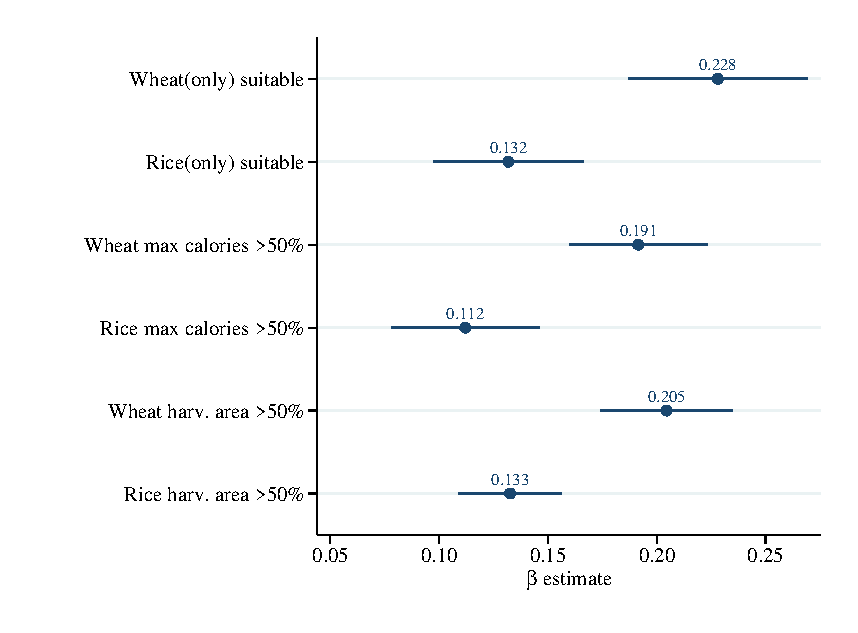
\includegraphics[width=0.9\textwidth]{fig_coef_crop_base.eps}
\end{center}
\hfill \hyperlink{cropreg}{\beamerbutton{Table}}
\end{frame}

\begin{frame}{Residual plot from baseline results}
\begin{center}
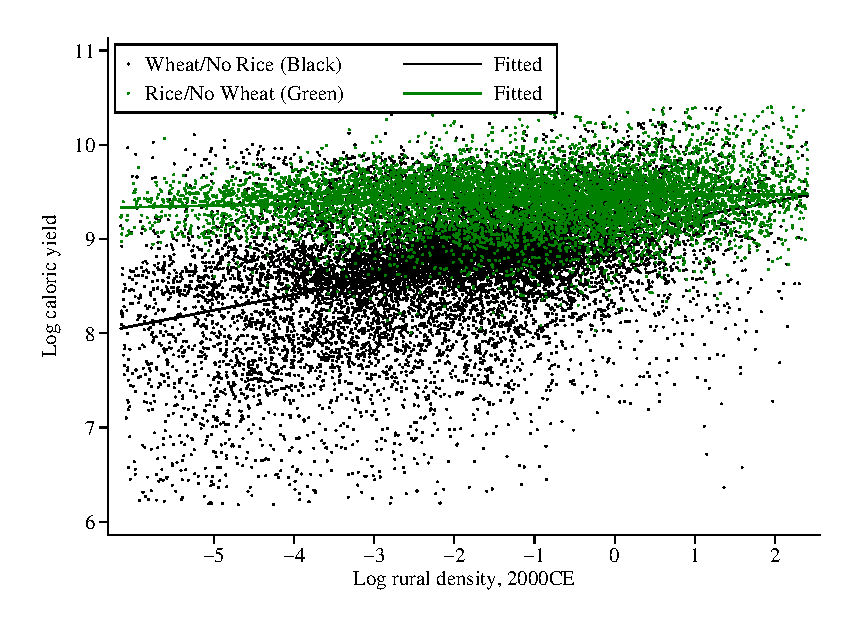
\includegraphics[width=.9\textwidth]{fig_beta_crop.eps}
\end{center}
\end{frame}

\begin{frame}{Results by Temperate/Tropical}
\begin{center}
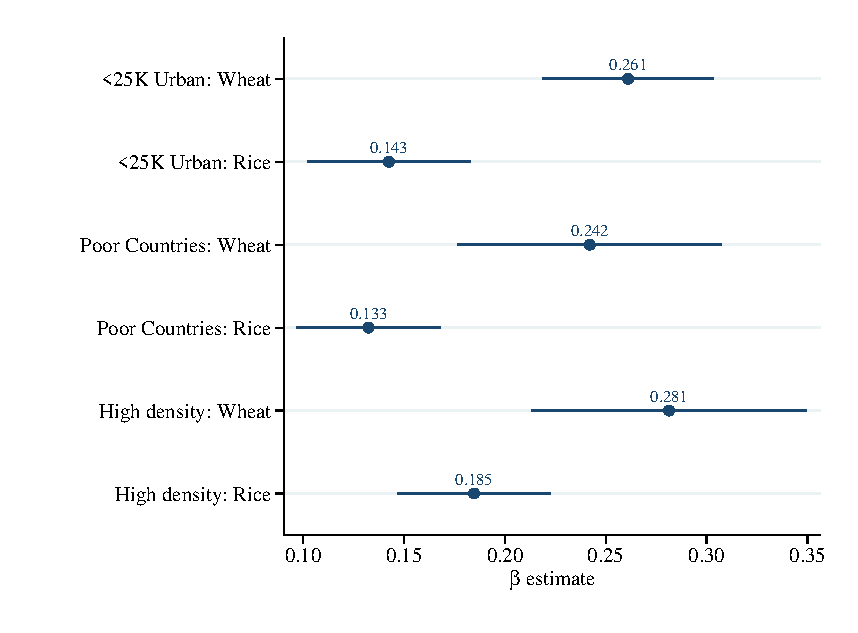
\includegraphics[width=.9\textwidth]{fig_coef_crop_sub_base.eps}
\end{center}
\end{frame}

\begin{frame}{Results using different population sources}\label{pop}
\begin{center}
\includegraphics[width=.9\textwidth]{fig_coef_robust_pop.eps}
\end{center}
\hfill \hyperlink{popreg}{\beamerbutton{Table}}
\end{frame}

\begin{frame}{Results using different land assumptions}\label{land}
\begin{center}
\includegraphics[width=.9\textwidth]{fig_coef_robust_other.eps}
\end{center}
\hfill \hyperlink{landreg}{\beamerbutton{Table}}
\end{frame}

\begin{frame}{Results using different $A^{GAEZ}_{isg}$ level}\label{prod}
\begin{center}
\includegraphics[width=.9\textwidth]{fig_coef_robust_input.eps}
\end{center}
\hfill \hyperlink{prodreg}{\beamerbutton{Table}}
\end{frame}

\begin{frame}{Questions and more robustness}\label{robustness}
\begin{itemize}
  \item Use province level data (with country FE) \hyperlink{regprov}{\beamerbutton{Results}}
  \item By political regions \hyperlink{subregiontab}{\beamerbutton{Results}}
  \item By Koppen-Geiger climate zone \hyperlink{climatereg}{\beamerbutton{Results}}
  \item Inclusive definitions of temp. and trop. \hyperlink{definition}{\beamerbutton{Results}}
  \item Use rural density for 1900 from HYDE \hyperlink{reg1900}{\beamerbutton{Results}}
  \item Workers not mobile between districts? \hyperlink{nonmobile}{\beamerbutton{Slides}}
  \item Districts autarkic? \hyperlink{autarky}{\beamerbutton{Slides}}  
  \item Elasticity of substitution? \hyperlink{eos}{\beamerbutton{Slides}}
  \item Measurement error? \hyperlink{measure}{\beamerbutton{Slides}}
  \item Factor shares? \hyperlink{shares}{\beamerbutton{Slides}}
\end{itemize}
\end{frame}

\section{Implications}

\begin{frame}{Back to the model}\label{extend}
\begin{itemize}
  \item Non-agricultural sector that uses capital and labor too, with TFP $A_N$
  \item Agricultural sector as before, with TFP $A_A$ (a combo of district $A_A$)
  \item Labor and capital mobile between ag and non-ag, and across districts
  \item Preferences (Boppart, 2014) with income elasticity $<1$, governed by parameters $\gamma$ and $\epsilon$
  \item Gives nice analytical solutions for $L_A/L$ and real income $y$
\end{itemize}

\end{frame}

\begin{frame}{Elasticities}
The elasticities of the agricultural labor share ($L_A/L$) and real income ($y$) with respect to various shocks,
\begin{enumerate}
  \item[(a)] Agricultural productivity ($A_A$): 
\begin{equation}
  \frac{\partial \ln L_A/L}{\partial \ln A_A} = - \frac{\gamma}{1-\beta\gamma} \quad \quad \frac{\partial \ln y}{\partial \ln A_A} = \frac{1}{1-\beta\gamma}
\end{equation}
  \item[(c)] Population ($L$): 
\begin{equation}
  \frac{\partial \ln L_A/L}{\partial \ln L} = \frac{\beta\gamma}{1-\beta\gamma} \quad \quad \frac{\partial \ln y}{\partial \ln L} = - \frac{\beta}{1-\beta\gamma}
\end{equation}
\end{enumerate}
are all increasing in absolute value with $\beta$.
\end{frame}

\begin{frame}{Speculative implications:}
Three settings where the Malthusian constraint might matter
\begin{itemize}
  \item \textbf{Effect of Black Death:} Large effects on European development (Voigtl{\"a}nder and Voth, 2013a,b) due to tight constraint? Similar epidemics in Asia w/o major changes due to loose constraint?
  \item \textbf{Involution:} Higher densities and output, but not living standards, in response to productivity (Geertz, 1963; Huang, 1990) due to loose constraint?
  \item \textbf{Response to agric. technology/inputs:} Necessary increase to match rich countries in TFP/inputs is larger with loose constraint (Eberhardt and Vollrath, 2016a,b)
\end{itemize}
\end{frame}

\begin{frame}{Empirical implications:}\label{aj}
Acemoglu and Johnson (2007) analysis of epidemiological transition:
\begin{itemize}
  \item WHO (and other) interventions lower mortality rates from many tropical diseases
  \item They find higher resulting population was negative for income per capita
  \item According to our theory, the negative effect should be \textit{bigger} for places with \textit{higher} land elasticity
  \item We divide countries in AJ into ``high'' and ``low'' $\beta$ groups based on country-specific elasticities, run AJ analysis separately for those groups
  \item Consistent with prediction, high $\beta$ countries had much larger negative effects on GDP per worker, GDP per capita in response to mortality decline
\end{itemize}

\hfill \hyperlink{mortality}{\beamerbutton{Tables}}
\end{frame}

\section{Conclusion}

\begin{frame}{Conclusion}
\begin{itemize}
  \item Estimate aggregate land elasticity from variation in rural density within provinces
  \item Elasticity is high (0.20-0.25) in temperate agricultural areas 
  \item Elasticity is low (0.10-0.15) in tropical agricultural areas 
  \item Elasticity affects the sensitivity of $L_A/L$ and living standards to population and productivity
  \item Evidence from epidemiological transition is consistent with our findings and theory
  \item Implications for the study of historical and contemporary development
\end{itemize}
\end{frame}

\section{Appendix Slides}
\appendix

\subsection{Additional information}
\begin{frame}{Interaction Regression}\label{interaction}
Combine a given sample with the reference sample (denoted by $Ref$). Run the following regression with interaction terms
\begin{eqnarray}
    \ln A_{isg} = \beta \ln L_{Aisg}/X_{isg} + (\beta^{Ref}_g - \beta_g) \ln L_{Aisg}/X_{isg} \times I(Ref) \\ \nonumber
    + \gamma_{s} + \delta_g' \mathbf{Z}_{isg} + (\delta^{Ref}_g - \delta_g)'\mathbf{Z}_{isg} \times I(Ref) + \epsilon_{isg}. \label{EQ_interaction}
\end{eqnarray}
where $I(Ref)$ is an indicator for the reference region. Our hypothesis test is $H_0: \beta^{Ref}_g - \beta_g = 0$, the coefficient on the interaction term for rural density. 

\hfill \hyperlink{testing}{\beamerbutton{Return}}
\end{frame}

\begin{frame}{Summary statistics}\label{stats}
{\scriptsize
\begin{tabularx}{\textwidth}{lXXXXXXX}
\midrule
 &      &            & \multicolumn{5}{c}{Percentiles:} \\ \cmidrule{4-8}
 & Mean & SD  & 10th    & 25th    & 50th & 75th & 90th \\
\midrule
Labor/land (persons/ha) &     0.73&     1.17&     0.04&     0.12&     0.32&     0.77&     1.86\\
Caloric yield (mil cals/ha) &    10.85&     4.89&     4.98&     7.17&    10.65&    13.86&    17.03\\
Log light density &    -2.82&     2.93&    -6.14&    -3.83&    -2.51&    -0.89&     0.35\\

\midrule
\end{tabularx}
}

\hfill \hyperlink{data}{\beamerbutton{Return}}
\end{frame}

\begin{frame}{Crops used in productivity calculation}\label{crops}
alfalfa, banana, barley, buckwheat, cassava, chickpea, cowpea, drypea, flax, foxtail millet, greengram, groundnut, indica rice, maize, oat, pearl millet, phaselous bean, pigeon pea, rye, sorghum, soybean, spring wheat, sweetpotato, rape, wet/paddy rice, wheat, winter wheat, white potato, and yams

\hfill \hyperlink{data}{\beamerbutton{Return}}
\end{frame}

\subsection{Main results}


\begin{frame}{Crop Results}\label{cropreg}
{\footnotesize
\begin{tabularx}{\textwidth}{lXXXXXX}
\midrule
\multicolumn{7}{l}{Dependent Variable in all panels: Log caloric yield ($A_{isc}$)} \\ \\
\multicolumn{7}{l}{Panel A: Samples defined by crop family (wheat vs. rice):} \\ \\
 & \multicolumn{2}{c}{By suitability:} & \multicolumn{2}{c}{By max calories:} & \multicolumn{2}{c}{By harvest area:}\\ \cmidrule(lr){2-3} \cmidrule(lr){4-5} \cmidrule(lr){6-7} 
 & Wheat & Rice & Wheat  & Rice  & Wheat  & Rice \\
 & Only & Only &  $>33\%$ & $>33\%$ & $>50\%$ & $>50\%$   \\
 & (1) & (2) & (3) & (4) & (5) & (6) \\
\midrule
Log labor/land ratio ($\beta_g$)&       0.239&       0.088&       0.218&       0.093&       0.220&       0.081\\
                    &     (0.045)&     (0.020)&     (0.039)&     (0.012)&     (0.049)&     (0.016)\\
\midrule
p-value $\beta_g=0$ &       0.000&       0.000&       0.000&       0.000&       0.000&       0.000\\
p-value $\beta_g=\beta_{Temp}$&            &       0.002&            &       0.002&            &       0.007\\
Countries           &          84&          76&          91&         101&          86&          78\\
Observations        &        9404&        7229&       15260&       14794&       10221&       10013\\
R-square (ex. FE)   &        0.24&        0.20&        0.21&        0.18&        0.23&        0.18\\

\midrule
\end{tabularx}
}

\hfill \hyperlink{crop}{\beamerbutton{Return}}
\end{frame}

\begin{frame}{Crop Results}

{\footnotesize
\begin{tabularx}{\textwidth}{lXXXXXX}
\midrule
\multicolumn{7}{l}{Dependent Variable in all panels: Log caloric yield ($A^{GAEZ}_{isg}$)} \\ \\
\multicolumn{7}{l}{Panel A: Regions defined by:} \\ \\
 & \multicolumn{2}{c}{Suitability:} & \multicolumn{2}{c}{Max calories:} & \multicolumn{2}{c}{Harvest area:}\\ \cmidrule(lr){2-3} \cmidrule(lr){4-5} \cmidrule(lr){6-7} 
 & Temperate & Tropical & Temperate  & Tropical  & Temperate  & Tropical \\
 & (1) & (2) & (3) & (4) & (5) & (6) \\
\midrule
Log labor/land ratio ($\beta_g$)&       0.239&       0.088&       0.218&       0.093&       0.220&       0.081\\
                    &     (0.045)&     (0.020)&     (0.039)&     (0.012)&     (0.049)&     (0.016)\\
\midrule
p-value $\beta_g=0$ &       0.000&       0.000&       0.000&       0.000&       0.000&       0.000\\
p-value $\beta_g=\beta_{Temp}$&            &       0.002&            &       0.002&            &       0.007\\
Countries           &          84&          76&          91&         101&          86&          78\\
Observations        &        9404&        7229&       15260&       14794&       10221&       10013\\
R-square (ex. FE)   &        0.24&        0.20&        0.21&        0.18&        0.23&        0.18\\

\midrule
\end{tabularx}
}
\end{frame}

\begin{frame}{Population results}\label{popreg}
{\footnotesize
\begin{tabularx}{\textwidth}{lXXXXXX}
\midrule
\multicolumn{7}{l}{Panel B: With other restrictions (using suitability to define temperate/tropical)} \\ \\
 & \multicolumn{2}{c}{Urban Pop. $<25K$:} & \multicolumn{2}{c}{Ex. Europe/N. Amer.:} & \multicolumn{2}{c}{Rural dens. $>$ 25th P'tile:}\\ \cmidrule(lr){2-3} \cmidrule(lr){4-5} \cmidrule(lr){6-7}
 & Temperate & Tropical & Temperate  & Tropical  & Temperate  & Tropical \\
 & (1) & (2) & (3) & (4) & (5) & (6) \\
\midrule
Residuals           &       0.257&       0.140&       0.223&       0.131&       0.215&       0.128\\
                    &     (0.022)&     (0.021)&     (0.032)&     (0.018)&     (0.021)&     (0.020)\\
\midrule
p-value $\beta=0$   &       0.000&       0.000&       0.000&       0.000&       0.000&       0.000\\
p-value $\beta=\beta_{Temp}$&            &       0.000&            &       0.009&            &       0.003\\
Countries           &          83&          75&          24&          70&          82&          66\\
Observations        &        7648&        6662&         824&        8826&        8084&        6611\\
Adjusted R-square   &        0.29&        0.24&        0.16&        0.14&        0.24&        0.20\\

\midrule
\end{tabularx}
}

\hfill \hyperlink{pop}{\beamerbutton{Return}}
\end{frame}


\begin{frame}{Land results}\label{landreg}
{\footnotesize
\begin{tabularx}{\textwidth}{lXXXXXX}
\midrule
\multicolumn{7}{l}{Dependent Variable in all panels: Log caloric yield ($A^{GAEZ}_{isg}$)} \\ \\
\multicolumn{7}{l}{Panel B: Different land assumptions} \\ \\
 & \multicolumn{2}{c}{Cultivated Area:} & \multicolumn{2}{c}{Drop $>$ 90th Ptile size:} & \multicolumn{2}{c}{Drop $<$ 25th Ptile Prod:}\\ \cmidrule(lr){2-3} \cmidrule(lr){4-5} \cmidrule(lr){6-7}
 & Temperate & Tropical & Temperate  & Tropical  & Temperate  & Tropical \\
 & (1) & (2) & (3) & (4) & (5) & (6) \\
\midrule
Log rural density ($\beta_g$)   &       0.215&       0.132&       0.215&       0.133&       0.239&       0.105\\
                    &     (0.020)&     (0.020)&     (0.020)&     (0.020)&     (0.028)&     (0.037)\\
\midrule
p-value $\beta_g=0$   &       0.000&       0.000&       0.000&       0.000&       0.000&       0.004\\
p-value $\beta_g=\beta_{Temp}$&            &       0.004&            &       0.004&            &       0.004\\
Countries           &          90&          78&          90&          78&          17&           5\\
Observations        &       10600&        8979&       10600&        8979&        3699&        2500\\
R-square (ex. FE)   &        0.26&        0.22&        0.26&        0.22&        0.33&        0.28\\

\midrule
\end{tabularx}
}

\hfill \hyperlink{land}{\beamerbutton{Return}}
\end{frame}


\begin{frame}{Productivity results}\label{prodreg}
{\footnotesize
\begin{tabularx}{\textwidth}{lXXXXXX}
\midrule
\multicolumn{7}{l}{Dependent Variable in all panels: Log caloric yield ($A^{GAEZ}_{isg}$)} \\ \\
\multicolumn{7}{l}{Panel A: Caloric yield based on GAEZ input/water use:} \\ \\
 & \multicolumn{2}{c}{Medium/Irrigated:} & \multicolumn{2}{c}{High/Rain-fed:} & \multicolumn{2}{c}{High/Irrigated:}\\ \cmidrule(lr){2-3} \cmidrule(lr){4-5} \cmidrule(lr){6-7} 
 & Temperate & Tropical & Temperate  & Tropical  & Temperate  & Tropical \\
 & (1) & (2) & (3) & (4) & (5) & (6) \\
\midrule
Log labor/land ratio ($\beta_g$)&       0.254&       0.120&       0.286&       0.132&       0.253&       0.120\\
                    &     (0.050)&     (0.022)&     (0.045)&     (0.025)&     (0.050)&     (0.022)\\
\midrule
p-value $\beta_g=0$ &       0.000&       0.000&       0.000&       0.000&       0.000&       0.000\\
p-value $\beta_g=\beta_{Temp}$&            &       0.014&            &       0.003&            &       0.014\\
Countries           &          72&          67&          72&          67&          72&          67\\
Observations        &        8416&        6731&        8389&        6719&        8416&        6731\\
R-square (ex. FE)   &        0.17&        0.14&        0.18&        0.14&        0.17&        0.14\\

\midrule
\end{tabularx}
}

\hfill \hyperlink{prod}{\beamerbutton{Return}}
\end{frame}

\begin{frame}{Productivity results}

{\footnotesize
\begin{tabularx}{\textwidth}{lXXXXXX}
\midrule
\multicolumn{7}{l}{Dependent Variable in all panels: Log caloric yield ($A^{GAEZ}_{isg}$)} \\ \\
\multicolumn{7}{l}{Panel B: Excluding N.A. and Europe, caloric yield based on GAEZ input/water use:} \\ \\
 & \multicolumn{2}{c}{Medium/Irrigated:} & \multicolumn{2}{c}{High/Rain-fed:} & \multicolumn{2}{c}{High/Irrigated:}\\ \cmidrule(lr){2-3} \cmidrule(lr){4-5} \cmidrule(lr){6-7} 
 & Temperate & Tropical & Temperate  & Tropical  & Temperate  & Tropical \\
 & (1) & (2) & (3) & (4) & (5) & (6) \\
\midrule
Residuals           &       0.236&       0.125&       0.235&       0.136&       0.238&       0.124\\
                    &     (0.037)&     (0.019)&     (0.039)&     (0.019)&     (0.034)&     (0.019)\\
\midrule
p-value $\beta=0$   &       0.000&       0.000&       0.000&       0.000&       0.000&       0.000\\
p-value $\beta=\beta_{Temp}$&            &       0.006&            &       0.017&            &       0.003\\
Countries           &          24&          70&          23&          69&          24&          70\\
Observations        &         824&        8826&         816&        8801&         824&        8826\\
Adjusted R-square   &        0.19&        0.15&        0.17&        0.13&        0.19&        0.15\\

\midrule
\end{tabularx}
}

\end{frame}


\begin{frame}{Climate Results}\label{climatereg}

{\footnotesize
\begin{tabularx}{\textwidth}{lXXXXXX}
\midrule
\multicolumn{7}{l}{Dependent Variable in all panels: Log caloric yield ($A_{isc}$)} \\ \\
\multicolumn{7}{l}{Panel A: Climate Zones} \\
 & Equatorial & Arid & Temperate & Snow  &     &   \\
 & (1) & (2) & (3) & (4) &  & \\
\midrule
Log labor/land ratio ($\beta_g$)&       0.142&       0.226&       0.207&       0.140&       0.190\\
                    &     (0.021)&     (0.053)&     (0.076)&     (0.035)&     (0.046)\\
\midrule
p-value $\beta=0$   &       0.000&       0.000&       0.007&       0.000&       0.000\\
p-value $\beta=\beta_{Humid}$&            &       0.065&       0.405&       0.969&       0.254\\
Countries           &          57&          82&          18&          42&          25\\
Observations        &        8101&        9003&         340&        1230&         956\\
R-square (ex. FE)   &        0.20&        0.23&        0.20&        0.17&        0.21\\

\midrule
\end{tabularx}
}

\hfill \hyperlink{robustness}{\beamerbutton{Return}}
\end{frame}

\begin{frame}{Climate Results}

{\footnotesize
\begin{tabularx}{\textwidth}{lXXXXXX}
\midrule
\multicolumn{7}{l}{Panel B: Precipitation Zones} \\
& Fully     & Dry         & Dry        &              &            & \\
& Humid & Summer & Winter & Monsoon & Desert & Steppe \\
 & (1) & (2) & (3) & (4) & (5) & (6) \\
\midrule
Log labor/land ratio ($\beta_g$)&       0.240&       0.215&       0.124&       0.125&       0.130&       0.147\\
                    &     (0.044)&     (0.063)&     (0.022)&     (0.039)&     (0.072)&     (0.029)\\
\midrule
p-value $\beta=0$   &       0.000&       0.001&       0.000&       0.001&       0.072&       0.000\\
p-value $\beta=\beta_{Humid}$&            &       0.739&       0.020&       0.043&       0.190&       0.072\\
Countries           &          78&          37&          67&          32&          20&          49\\
Observations        &       13545&        2373&        7695&        1267&         146&        1735\\
R-square (ex. FE)   &        0.17&        0.17&        0.15&        0.17&        0.17&        0.16\\

\midrule
\end{tabularx}
}

\end{frame}

\begin{frame}{Climate Results}

{\footnotesize
\begin{tabularx}{\textwidth}{lXXXXXX}
\midrule
\multicolumn{7}{l}{Panel C: Temperature Zones} \\
    & Hot        & Warm        & Cool       & Hot      & Cold     &  \\
    & Summer & Summer & Summer & Arid & Arid &   \\
 & (1) & (2) & (3) & (4) & (5) &  \\    
\midrule
Log labor/land ratio ($\beta_g$)&       0.142&       0.226&       0.207&       0.140&       0.190\\
                    &     (0.021)&     (0.053)&     (0.076)&     (0.035)&     (0.046)\\
\midrule
p-value $\beta=0$   &       0.000&       0.000&       0.007&       0.000&       0.000\\
p-value $\beta=\beta_{Humid}$&            &       0.065&       0.405&       0.969&       0.254\\
Countries           &          57&          82&          18&          42&          25\\
Observations        &        8101&        9003&         340&        1230&         956\\
R-square (ex. FE)   &        0.20&        0.23&        0.20&        0.17&        0.21\\

\midrule
\end{tabularx}
}
\end{frame}

\begin{frame}{Region Results}\label{subregiontab}

{\footnotesize
\begin{tabularx}{\textwidth}{lXXXXX}
\midrule
\multicolumn{6}{l}{Dependent Variable in all panels: Log caloric yield ($A_{isc}$)} \\ \\
\multicolumn{6}{l}{Panel A} \\
 &          &         &             &  \multicolumn{2}{c}{Excl. China, Japan, Korea} \\ \cmidrule(lr){5-6}
 & North \& &         &              & South \&  & Central \&             \\
 & Western  & Eastern & Southern     & Southeast & West        \\
 & Europe   & Europe  & Europe       & Asia      & Asia      \\
 & (1) & (2) & (3) & (4) & (5) \\
\midrule
Log rural density ($\beta_g$)&       0.259&       0.287&       0.272&       0.152&       0.181\\
                    &     (0.036)&     (0.031)&     (0.041)&     (0.026)&     (0.024)\\
\midrule
p-value $\beta=0$   &       0.000&       0.000&       0.000&       0.000&       0.000\\
p-value $\beta=\beta_{NWEur}$&            &       0.539&       0.791&       0.017&       0.072\\
Countries           &          16&           9&           9&          13&          18\\
Observations        &        1684&        4821&        1137&        4312&        2878\\
R-square (ex. FE)   &        0.29&        0.34&        0.32&        0.21&        0.24\\

\midrule
\end{tabularx}
}

\hfill \hyperlink{robustness}{\beamerbutton{Return}}
\end{frame}

\begin{frame}{Region Results}

{\footnotesize
\begin{tabularx}{\textwidth}{lXXXXX}
\midrule
\multicolumn{6}{l}{Dependent Variable in all panels: Log caloric yield ($A_{isc}$)} \\ \\
\multicolumn{6}{l}{Panel B} \\
 & Temperate & Tropical  & Tropical & South    & North    \\
 & Americas  & Americas  & Africa   & Africa   & Africa     \\
\midrule
Residuals           &       0.188&       0.113&       0.089&       0.134&       0.249\\
                    &     (0.030)&     (0.016)&     (0.014)&     (0.071)&     (0.014)\\
\midrule
p-value $\beta=0$   &       0.000&       0.000&       0.000&       0.059&       0.000\\
p-value $\beta=\beta_{NWEur}$&       0.133&       0.000&       0.000&       0.116&       0.827\\
Countries           &           5&          22&          39&           4&           5\\
Observations        &        3796&        9373&        3181&         198&        1220\\
R-square (ex. FE)   &        0.24&        0.12&        0.18&        0.27&        0.28\\

\midrule
\end{tabularx}
}

\end{frame}

\begin{frame}{Region Results}

{\footnotesize
\begin{tabularx}{\textwidth}{lXXXXX}
\midrule
\multicolumn{6}{l}{Dependent Variable in all panels: Log caloric yield ($A_{isc}$)} \\ \\
\multicolumn{6}{l}{Panel C} \\
 & All& Temperate & Sub-Tropical & & North \& \\
 & China & China  & China & Japan & South Korea  \\
 & (1) & (2) & (3) & (4) & (5) \\
\midrule
Log rural density   &       0.414&       0.518&       0.107&       0.155&       0.190\\
                    &     (0.083)&     (0.058)&     (0.026)&     (0.011)&     (0.061)\\
\midrule
p-value $\beta=0$   &       0.000&       0.000&       0.000&       0.000&       0.002\\
p-value $\beta=\beta^{NWEur}$&       0.102&       0.000&       0.001&       0.008&       0.309\\
Countries           &           1&           1&           1&           1&           2\\
Observations        &         266&         130&         136&        1039&         311\\
Adjusted R-square   &        0.25&        0.26&        0.21&        0.21&        0.21\\

\midrule
\end{tabularx}
}

\end{frame}

\begin{frame}{Results by Region}
\begin{center}
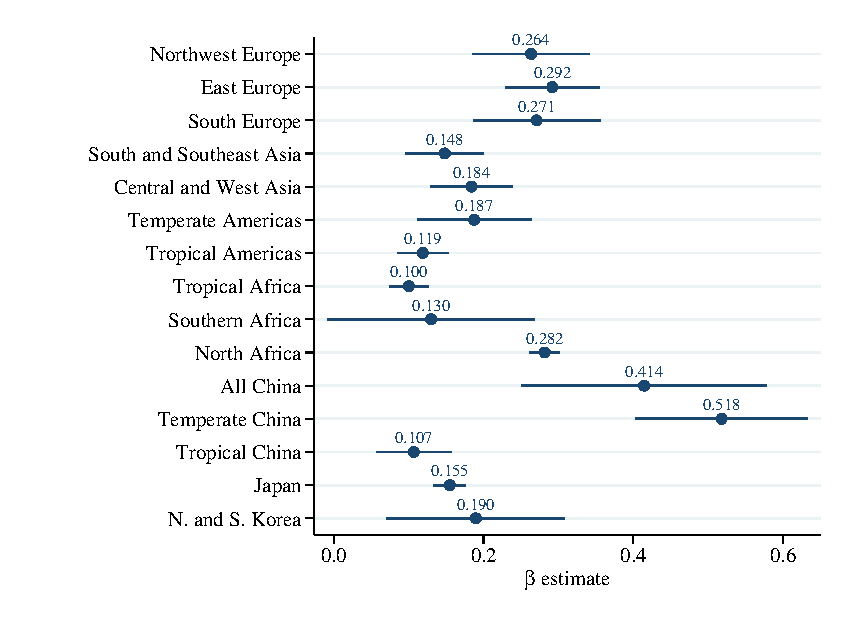
\includegraphics[width=.8\textwidth]{fig_coef_subregion_base.eps}
\end{center}
\end{frame}


\subsection{Robustness checks}

\begin{frame}{Results by Province}\label{prov}
Baseline results assume $\beta$ constant within larger sub-samples. 

\vspace{.2cm}Instead, estimate $\beta$ individually for each province
\begin{itemize}
  \item Only provinces with 6 or more districts (1,260 provinces)
  \item ... so really big SE on any individual estimate
  \item Then look at pattern of $\beta$'s for each sub-sample
\end{itemize}
\end{frame}

\begin{frame}{Results by Province}

{\scriptsize
\begin{tabularx}{\textwidth}{lrrrXXXXX}
\midrule
           &       &      &     & \multicolumn{5}{c}{Percentiles:} \\ \cmidrule{5-9}
Sample & Prov. & Mean & SD  & 10th    & 25th    & 50th & 75th & 90th \\
\midrule
All provinces &    1,183&     0.21&     0.23&    -0.02&     0.05&     0.18&     0.33&     0.49\\ \\
Wheat Suitable &      619&     0.23&     0.23&    -0.00&     0.08&     0.21&     0.36&     0.50\\
Rice Suitable &      469&     0.17&     0.24&    -0.04&     0.03&     0.15&     0.28&     0.43\\
Wheat cals>33\% &      457&     0.23&     0.22&    -0.00&     0.08&     0.21&     0.36&     0.50\\
Rice cals>33\% &      307&     0.18&     0.21&    -0.04&     0.03&     0.15&     0.29&     0.41\\
Wheat area>50\% &      485&     0.22&     0.23&    -0.01&     0.07&     0.20&     0.36&     0.53\\
Rice area>50\% &      297&     0.18&     0.23&    -0.04&     0.03&     0.14&     0.29&     0.47\\ \\
Northwest Europe &        79&     0.26&     0.31&     0.00&     0.08&     0.22&     0.46&     0.62\\
Eastern Europe &       173&     0.24&     0.20&     0.01&     0.09&     0.23&     0.38&     0.50\\
Southern Europe &        60&     0.27&     0.17&     0.08&     0.16&     0.25&     0.37&     0.50\\
South and S. East Asia &       248&     0.20&     0.23&    -0.03&     0.04&     0.16&     0.31&     0.49\\
Central and West. Asia &       163&     0.20&     0.20&    -0.02&     0.06&     0.16&     0.33&     0.45\\
Temperate Americas &        87&     0.14&     0.25&    -0.13&     0.02&     0.10&     0.26&     0.40\\
Tropical Americas &       195&     0.18&     0.26&    -0.02&     0.06&     0.17&     0.28&     0.39\\
Tropical Africa &       118&     0.16&     0.24&    -0.09&    -0.01&     0.09&     0.25&     0.51\\
Southern Africa &        11&     0.15&     0.21&    -0.11&    -0.05&     0.17&     0.33&     0.34\\
Northern Africa &        49&     0.32&     0.20&     0.06&     0.22&     0.31&     0.42&     0.66\\

\midrule
\end{tabularx}
}

\hfill \hyperlink{robustness}{\beamerbutton{Return}}
\end{frame}

\begin{frame}{Results by Province}
\begin{center}
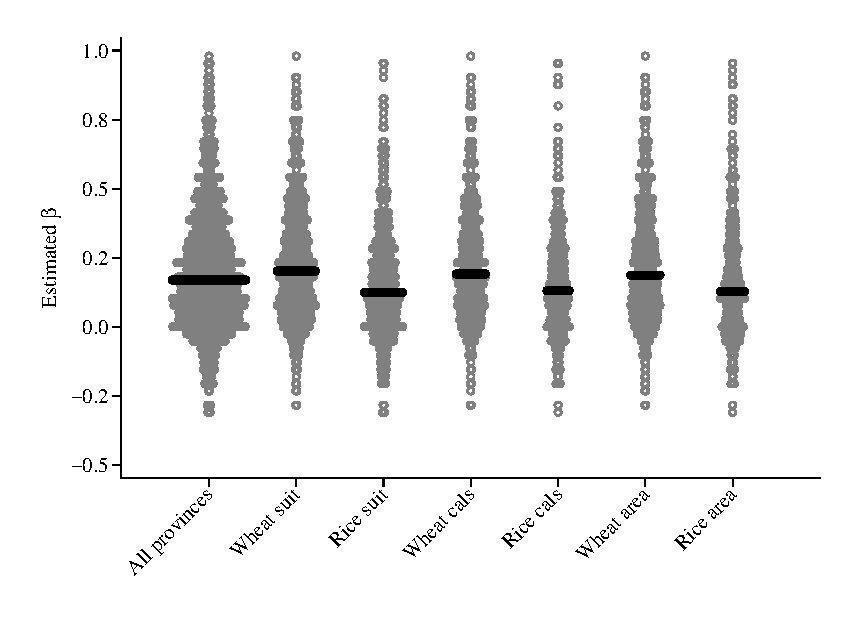
\includegraphics[width=.8\textwidth]{fig_beta_province.eps}
\end{center}
\end{frame}

\begin{frame}{Relationship of $\beta$ to rural density, by province}\label{rurdbeta}
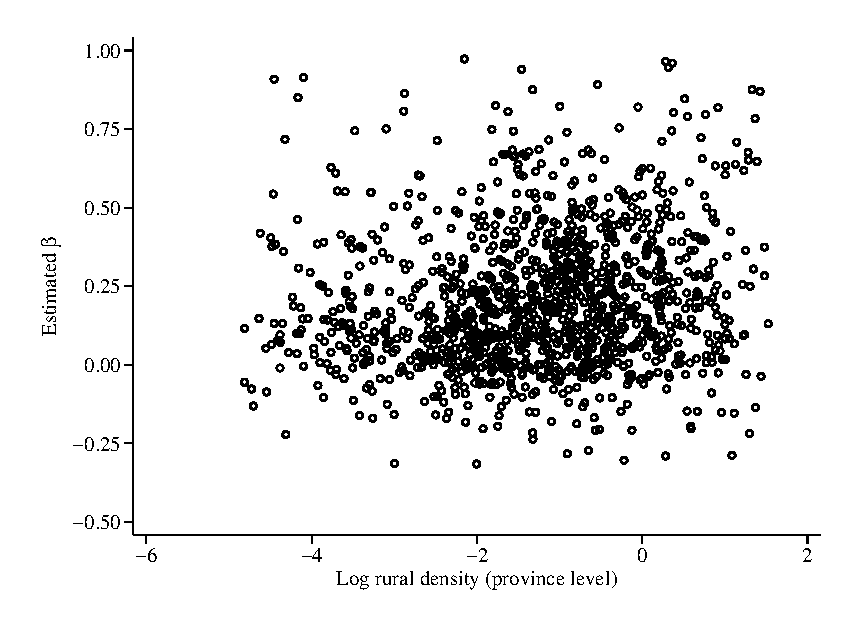
\includegraphics[width=.8\textwidth]{fig_beta_rurd.eps}
\hfill \hyperlink{eos}{\beamerbutton{Return}}
\end{frame}

\begin{frame}{Labor and capital not mobile}\label{nonmobile}
Factors cannot move within province, but output can.

\vspace{.2cm} Changes relationship of density and productivity to
\begin{equation}
  \ln A_{Ai} = \beta \ln L_{Ai}/X_i + \ln A_{Ni} + \alpha\beta \ln K_i/L_i + \ln p_N/p_A \nonumber
\end{equation}
\begin{itemize}
  \item Night lights provide proxy for $A_{Ni}$ and $K_i/L_i$?
  \item $p_N/p_A$ is province-specific (FE)
  \item Is correlation of $A_{Ni}$ and $K_i/L_i$ with $L_{Ai}/X_i$ different by climate zone?
\end{itemize}

\hfill \hyperlink{robustness}{\beamerbutton{Return}}
\end{frame}

\begin{frame}{Districts are autarkic}\label{autarky}
Factors and output are immobile within province.

\vspace{.2cm} Changes relationship of density and productivity to
\begin{equation}
\ln A_i = \beta \ln L_{Ai}/X_i - \ln L_{A_i}/L_i - \alpha(1-\beta) \ln K_{i}/L_{i} + \ln c_{Ai} \nonumber
\end{equation}
\begin{itemize}
  \item Can control for $L_{Ai}/L_i$ using HYDE data
  \item Night lights provide proxy for $K_i/L_i$?
  \item $c_{Ai}$ doesn't vary much and/or proxied by night lights?
\end{itemize}

\hfill \hyperlink{robustness}{\beamerbutton{Return}}
\end{frame}


\begin{frame}{Using Cultivated Area}\label{cultivated}
Cultivated area, $X^C_{isc}$, available from GAEZ. Rural density is
\begin{equation}
  \ln L_{Aisc}/X_{isc} = \ln L_{Aisc}/X^C_{isc} + \ln X^C_{isc}/X_{isc}
\end{equation}

\begin{itemize}
  \item Regress $\ln A_{isc}$ on both terms on the right hand-side 
  \item Coefficient on $\ln L_{Aisc}/X^C_{isc}$ gives similar results for $\beta$
  \item Controls for percent of land actually being cultivated
\end{itemize}

\hfill \hyperlink{land}{\beamerbutton{Return}}
\end{frame}

\begin{frame}{Measurement error?}
\begin{itemize}
  \item Whether we are using cultivated or total area
  \item Systematic mismeasurement of districts within a province not a problem, FE
  \item Variation in systematic mismeasurement across provinces not a problem, FE
  \item Problem is \textit{variation in noise of mismeasurement} across provinces
  \item Is there noisier measurement in tropical areas? 
\end{itemize}
\end{frame}


\begin{frame}{Province-level Data}\label{regprov}

{\footnotesize
\begin{tabularx}{\textwidth}{lXXXXXX}
\midrule
\multicolumn{7}{l}{Dependent Variable in all panels: Log caloric yield ($A_{isc}$)} \\ \\
\multicolumn{7}{l}{Panel A: Samples defined by crop family (wheat vs. rice):} \\ \\
 & \multicolumn{2}{c}{By suitability:} & \multicolumn{2}{c}{By max calories:} & \multicolumn{2}{c}{By harvest area:}\\ \cmidrule(lr){2-3} \cmidrule(lr){4-5} \cmidrule(lr){6-7} 
 & Wheat & Rice & Wheat  & Rice  & Wheat  & Rice \\
 & Only & Only &  $>33\%$ & $>33\%$ & $>50\%$ & $>50\%$   \\
 & (1) & (2) & (3) & (4) & (5) & (6) \\
\midrule
Log rural density   &       0.399&       0.070&       0.248&       0.016&       0.368&       0.052\\
                    &     (0.058)&     (0.020)&     (0.030)&     (0.013)&     (0.043)&     (0.021)\\
\midrule
p-value $\beta=0$   &       0.000&       0.000&       0.000&       0.199&       0.000&       0.014\\
p-value $\beta=\beta^{Wheat}$&            &       0.000&            &       0.000&            &       0.000\\
Countries           &          60&          65&          70&          63&          69&          73\\
Observations        &         417&         587&         768&         617&         797&         721\\
Adjusted R-square   &        0.39&        0.27&        0.29&        0.26&        0.35&        0.30\\

\midrule
\end{tabularx}
}

\hfill \hyperlink{robustness}{\beamerbutton{Return}}
\end{frame}

\begin{frame}{Population Data from 1900}\label{reg1900}

{\footnotesize
\begin{tabularx}{\textwidth}{lXXXXXX}
\midrule
\multicolumn{7}{l}{Dependent Variable in all panels: Log caloric yield ($A_{isc}$)} \\ \\
\multicolumn{7}{l}{Panel A: Samples defined by crop family (wheat vs. rice):} \\ \\
 & \multicolumn{2}{c}{By suitability:} & \multicolumn{2}{c}{By max calories:} & \multicolumn{2}{c}{By harvest area:}\\ \cmidrule(lr){2-3} \cmidrule(lr){4-5} \cmidrule(lr){6-7} 
 & Wheat & Rice & Wheat  & Rice  & Wheat  & Rice \\
 & Only & Only &  $>33\%$ & $>33\%$ & $>50\%$ & $>50\%$   \\
 & (1) & (2) & (3) & (4) & (5) & (6) \\
\midrule
Log rural density   &       0.294&       0.170&       0.239&       0.149&       0.258&       0.182\\
                    &     (0.032)&     (0.025)&     (0.023)&     (0.025)&     (0.026)&     (0.017)\\
\midrule
p-value $\beta=0$   &       0.000&       0.000&       0.000&       0.000&       0.000&       0.000\\
p-value $\beta=\beta^{Wheat}$&            &       0.002&            &       0.007&            &       0.014\\
Countries           &          91&          81&          83&          71&          74&          84\\
Observations        &       10644&        9081&       10774&        8213&       10689&        7561\\
Adjusted R-square   &        0.30&        0.25&        0.25&        0.22&        0.24&        0.22\\

\midrule
\end{tabularx}
}

\hfill \hyperlink{robustness}{\beamerbutton{Return}}
\end{frame}

\begin{frame}{Above 25th Percentile Harvested Area}\label{harvarea}

{\footnotesize
\begin{tabularx}{\textwidth}{lXXXXXX}
\midrule
\multicolumn{7}{l}{Dependent Variable in all panels: Log caloric yield ($A_{isc}$)} \\ \\
\multicolumn{7}{l}{Panel A: Samples defined by crop family (wheat vs. rice):} \\ \\
 & \multicolumn{2}{c}{By suitability:} & \multicolumn{2}{c}{By max calories:} & \multicolumn{2}{c}{By harvest area:}\\ \cmidrule(lr){2-3} \cmidrule(lr){4-5} \cmidrule(lr){6-7} 
 & Wheat & Rice & Wheat  & Rice  & Wheat  & Rice \\
 & Only & Only &  $>33\%$ & $>33\%$ & $>50\%$ & $>50\%$   \\
 & (1) & (2) & (3) & (4) & (5) & (6) \\
\midrule
Log rural density   &       0.226&       0.140&       0.186&       0.111&       0.213&       0.125\\
                    &     (0.025)&     (0.020)&     (0.017)&     (0.021)&     (0.018)&     (0.013)\\
\midrule
p-value $\beta=0$   &       0.000&       0.000&       0.000&       0.000&       0.000&       0.000\\
p-value $\beta=\beta^{Wheat}$&            &       0.008&            &       0.005&            &       0.000\\
Countries           &          82&          65&          77&          58&          70&          72\\
Observations        &        7568&        6092&        7540&        5374&        8400&        5704\\
Adjusted R-square   &        0.22&        0.18&        0.19&        0.16&        0.19&        0.16\\

\midrule
\end{tabularx}
}

\hfill \hyperlink{robustness}{\beamerbutton{Return}}
\end{frame}

\begin{frame}{Other definitions of temperate and tropical}\label{definition}

{\footnotesize
\begin{tabularx}{\textwidth}{lXXXXXX}
\midrule
\multicolumn{6}{l}{Dependent Variable: Log caloric yield ($A_{isg}$)} \\ \\
 &   & &                             & \multicolumn{3}{c}{Urban Pop. $<25K$} \\
 & \multicolumn{3}{c}{Suitable for:} & \multicolumn{3}{c}{Suitable for:} \\ \cmidrule(lr){2-4} \cmidrule(lr){5-7}
 & Temperate   & Any       & Any      & Temperate     & Any       & Any      \\
 & and Tropical & Temperate & Tropical & and Tropical & Temperate & Tropical \\
 & (1) & (2) & (3) & (4) & (5) & (6) \\
\midrule
Log rural density   &       0.140&       0.180&       0.132&       0.156&       0.202&       0.145\\
                    &     (0.013)&     (0.017)&     (0.011)&     (0.015)&     (0.020)&     (0.013)\\
\midrule
p-value $\beta=0$   &       0.000&       0.000&       0.000&       0.000&       0.000&       0.000\\
Countries           &         119&         137&         137&         110&         131&         130\\
Observations        &       15692&       26353&       24780&       11008&       18656&       17670\\
Adjusted R-square   &        0.13&        0.18&        0.12&        0.15&        0.20&        0.14\\

\midrule
\end{tabularx}
}

\hfill \hyperlink{robustness}{\beamerbutton{Return}}
\end{frame}




\begin{frame}{Measurement Error}\label{measure}
Measurement error $\Rightarrow$ attentuation bias
\begin{itemize}
  \item Population data from HYDE may not be accurate for districts
  \item Is measurement error more pronounced in some places (e.g. tropical areas) and driving results?
  \item Is true variance of $\ln L_{Aisc}/X_{isc}$ one-third of measured variance?
  \item Is rural population mis-stated by factor of $>2$ or $<0.5$?
\end{itemize}

\hfill \hyperlink{robustness}{\beamerbutton{Return}}
\end{frame}

\begin{frame}{Elasticity of Substitution?}\label{eos}
What if land and labor do not have elasticity of subs. equal to one?
\begin{itemize}
  \item Elasticity of output w.r.t. land depends on rural density $L_A/X$
  \item With EOS more than one, higher density, lower elasticity
  \item Do results fit this?
  \begin{itemize}
    \item South/SE Asia, some SS Afr are high density, low $\beta$
    \item ..but C/S America, other SS Afr are low density, low $\beta$
    \item ..but N America lowest density, not highest $\beta$
  \end{itemize}
\end{itemize}
\hfill \hyperlink{rurdbeta}{\beamerbutton{Density?}}
\hfill \hyperlink{robustness}{\beamerbutton{Return}}
\end{frame}

\begin{frame}{Factor shares}\label{shares}
Our $\beta$ does not correlate well with factor share data
\begin{itemize}
  \item Fuglie (2010) reports share for ``land and structures''
  \begin{itemize}
    \item 0.22-0.25 share for Brazil, India, Indonesia $>$ our estimates
    \item 0.22 share for China, aggregate number?
    \item 0.17-0.26 for US, ex-Soviet $\approx$ our estimates
  \end{itemize}
  \item Hayami, Ruttan, Southworth (1979) for Asia
    \begin{itemize}
      \item 0.3-0.4 shares for Taiwan, Japan, Korea, Philippines $>$ our estimates
    \end{itemize}
  \item Clark (2002) for England, long run
    \begin{itemize}
      \item 0.3-0.35 shares $>$ our estimate for Northwest Europe
    \end{itemize}
\end{itemize}
\end{frame}

\begin{frame}{Factor Shares}
Possible sources of difference
\begin{itemize}
  \item Biased estimates of $\beta$
  \item Market frictions/wedges for agricultural inputs
  \item Mis-reporting of land versus labor income
  \item Difference of aggregate elasticity from farm-specific elasticity/share
\end{itemize}

\hfill \hyperlink{robustness}{\beamerbutton{Return}}
\end{frame}

\begin{frame}{Using GRUMP Population Data}\label{grump}
GRUMP (Global Rural-Urban Mapping Project) also provides grid-cell population estimates. 
\begin{itemize}
  \item Define urban/rural differently than HYDE. They denote specific grid-cells as ``urban'', and any population in that cell is assumed to be urban.
  \item Inclusion of cells in districts and provinces is identical to HYDE. 
\end{itemize}

\end{frame}

\begin{frame}{Using IPUMS Population Data}\label{ipums}
39 countries in IPUMS with geographic identifiers for individuals at the ``district'' level (agglomerations of districts with constant boundaries). 
\begin{itemize}
  \item IPUMS gives industry/occupation and labor force status, so we can measure \textit{agricultural worker density}, not just rural density. In practice, rural density and ag worker density correlated at 91\%, sig at less than 1\%
  \item Counts of residents in each district are presumably more accurate that HYDE or GRUMP, as they are drawn from census. 
  \item Cost is limited coverage of countries, and fewer districts
  \item Rebuild data on $A_{isc}$ and $L_{Aisc}$ at the level of the IPUMS districts
\end{itemize}

\hfill \hyperlink{pop}{\beamerbutton{Return}}
\end{frame}


\begin{frame}{Response to mortality rate changes}\label{mortality}

{\footnotesize
\begin{tabularx}{\textwidth}{lXXXXXX}
\midrule
 & \multicolumn{6}{c}{Dependent Variable:} \\ \cmidrule(lr){2-7}
 & \multicolumn{2}{c}{Log GDP per capita} & \multicolumn{2}{c}{Log GDP per worker} & \multicolumn{2}{c}{Log population} \\ \cmidrule(lr){2-3} \cmidrule(lr){4-5} \cmidrule(lr){6-7}
 & $\beta<$Median & $\beta>$Median & $\beta<$Median & $\beta>$Median & $\beta<$Median & $\beta>$Median \\
 & (1) & (2) & (3) & (4) & (5) & (6) \\
\midrule
 & \multicolumn{6}{c}{Panel A:} \\ \cmidrule(lr){2-7}
Mortality rate      &       0.333&       0.723&       0.284&       0.776&      -0.361&      -0.597\\
                    &     (0.271)&     (0.136)&     (0.262)&     (0.145)&     (0.186)&     (0.152)\\
\midrule
p-value $\theta=0$  &       0.220&       0.000&       0.281&       0.000&       0.054&       0.000\\
p-value $\theta=\theta^{Loose}$&           .&       0.199&           .&       0.102&           .&       0.327\\
Countries           &          16&          16&          16&          16&          16&          16\\
Observations        &         128&         128&         128&         128&         128&         128\\

\midrule

\end{tabularx}
}
\end{frame}

\begin{frame}{Response to life expectancy changes}

{\footnotesize
\begin{tabularx}{\textwidth}{lXXXXXX}
\midrule
 & \multicolumn{6}{c}{Dependent Variable:} \\ \cmidrule(lr){2-7}
 & \multicolumn{2}{c}{Log GDP per capita} & \multicolumn{2}{c}{Log GDP per worker} & \multicolumn{2}{c}{Log population} \\ \cmidrule(lr){2-3} \cmidrule(lr){4-5} \cmidrule(lr){6-7}
 & $\beta<$Median & $\beta>$Median & $\beta<$Median & $\beta>$Median & $\beta<$Median & $\beta>$Median \\
 & (1) & (2) & (3) & (4) & (5) & (6) \\
\midrule
 & \multicolumn{6}{c}{Panel B:} \\ \cmidrule(lr){2-7}
Log life expectancy &       0.309&      -2.007&       0.214&      -1.928&       1.910&       1.564\\
                    &     (0.393)&     (0.308)&     (0.387)&     (0.309)&     (0.235)&     (0.229)\\
\midrule
p-value $\theta=0$  &       0.434&       0.000&       0.582&       0.000&       0.000&       0.000\\
p-value $\theta=\theta^{Below}$&           .&       0.000&           .&       0.000&           .&       0.292\\
Countries           &          13&          14&          13&          14&          13&          14\\
Observations        &          99&         106&          99&         106&          99&         106\\

\midrule

\end{tabularx}
}
\end{frame}

\begin{frame}{Response to population change}

{\footnotesize
\begin{tabularx}{\textwidth}{lXXXXXX}
\midrule
 & \multicolumn{6}{c}{Dependent Variable:} \\ \cmidrule(lr){2-7}
 & \multicolumn{2}{c}{Log GDP per capita} & \multicolumn{2}{c}{Log GDP per worker} & \multicolumn{2}{c}{Log population} \\ \cmidrule(lr){2-3} \cmidrule(lr){4-5} \cmidrule(lr){6-7}
 & $\beta<$Median & $\beta>$Median & $\beta<$Median & $\beta>$Median & $\beta<$Median & $\beta>$Median \\
 & (1) & (2) & (3) & (4) & (5) & (6) \\
\midrule
 & \multicolumn{6}{c}{Panel C:} \\ \cmidrule(lr){2-7}
Log population      &      -0.380&      -0.776&      -0.383&      -0.763\\
                    &     (0.125)&     (0.067)&     (0.121)&     (0.062)\\
\midrule
p-value $\theta=0$  &       0.003&       0.000&       0.002&       0.000\\
p-value $\theta=\theta^{Below}$&           .&       0.006&           .&       0.006\\
Countries           &          16&          16&          16&          16\\
Observations        &         128&         128&         128&         128\\

\midrule

\end{tabularx}
}

\hfill \hyperlink{aj}{\beamerbutton{Return}}
\end{frame}


\end{document}
